\PassOptionsToPackage{dvispnames}{xcolor}
\documentclass[aspectratio=169]{beamer}
\usetheme[institute]{tugraz2018}
\usepackage[beamer]{prettytex/base}
\usepackage{prettytex/math}

\newcommand\labelenumi{\theenumi.}
\newcommand\labelenumii{(\theenumii)}
\newcommand\labelenumiii{\theenumiii.}
\newcommand\labelenumiv{\theenumiv.}

\title[Secure Classification as a Service]{
  Secure Classification as a Service \\
  \small\normalfont\textcolor{black}{
    Levelled Homomorphic, Post-Quantum Secure Machine Learning Inference \\
    based on the CKKS Encryption Scheme
  }
}
\author{Peter Waldert}
\date{Bachelor Thesis Presentation, 01.08.2022}
\institute{IAIK}
\instituteurl{iaik.tugraz.at}

\institutelogo{beamerthemetugraz/institute/IAIK}
% \additionallogo{figures/logo}  % additional institute/department logo (footline; optional)
% \logobar{Supported by: ...}  % sponsors (titlepage; optional)

\begin{document}
  \begin{frame}[plain]
    \maketitle
  \end{frame}

  \begin{frame}{Outline}
    \tableofcontents
  \end{frame}

  \section{Introduction}
  \begin{frame}{The frame title}
    A text frame
  \end{frame}

  \section{Content}
  \begin{frame}{Lists}
    \begin{itemize}
      \item First item
      \item Second item
      \item Third item
    \end{itemize}
  \end{frame}

  \begin{frame}{Numbered Lists and Pauses}
    \begin{enumerate}
      \item First item
            \begin{enumerate}
              \item First subitem
                    \begin{enumerate}
                      \item First
                      \item Second
                    \end{enumerate}
            \end{enumerate}
            \pause
      \item Second item
            \pause
      \item Third item
    \end{enumerate}
  \end{frame}

  \begin{frame}{An Image}
    \centering
    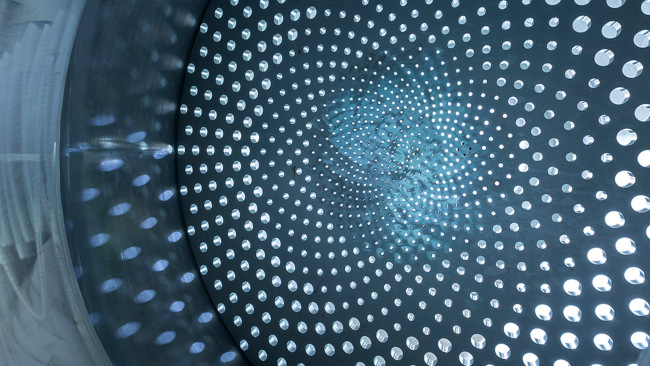
\includegraphics[height=0.6\textheight]{figures/photoexample-169}
  \end{frame}

  \section*{}
  \begin{frame}{Conclusion}
    ...
  \end{frame}

  %\begin{frame}[c,plain]
  \begin{frame}[c]
    \centering
    \Large Questions?
  \end{frame}
\end{document}
